\section{Introduction}
In this chapter we are going to present some of the recent work and research that was done regarding skin cancer detection and classification using machine learning , we are going to explore the various methods, tools, new ideas and challenges that was handeled by researchers for the hope of getting a clear understanding of the problem and how to go about solving it depending on each one's conditions, requirements and goals.



\section{skin cancer detection and classification using machine learning}
\begin{description}
    \item [proposed methodology]
    the proposed methodology in this article ~\cite{Krishna2020} uses a 6 step process (input data - preprocessing - segmentation - feature extraction - classification - output data)
    \item [input data] 
        dermoscopic images from the ISIC ( International Skin Imaging Collaboration) 2019 challenge containing 8 classes of skin cancer, and for simplisity reasons only 800 images out of 25000 is used.
    
    \item [preprocessing]
        because of the heteroginity of the input data a preprocessing step is required to inhance the quality of images and remove irrelevant parts. the main technices used here are gray scale conversion and the application of the Gaussian and median filter for noise removal and enhancement, and for the unwanted hair they applied the Dull Razor method (a preprocessing algorithm), as shown in figure ~\ref{fig:Preprocessing}

    \item [segmentation]
        segmnetation is used to extract the region of interest and for that they used a k-means clustering algorithm as shown in figure \ref{fig:segmentation}
        
    \item [feature extraction]
        for this they used 2 well know methods, ABCD method and GLCM. ABCD is used in dermatological applications and diagnosis for skin lesions such as melanomas and it is the abreviation of Asymmetry, Border, Color and Diameter. Grey Level Co-occurrence Matrix (GLCM) is used for texture analysis, other features are also used in addition to these 2 methods for further classification such as Autocorrelation, correlation, Standard vector...etc
    
    \item [classification]
        for classification they used MSVM (Multi-class Support vector machine) machine learning algorithm, they used trainning and testing ratios of 70:30 and obtained an acuuracy of 96.25\% and the confusion matrix shown in figure \ref{fig:confusion-matrix}
\end{description}

\begin{figure}[htbp]
\begin{center}
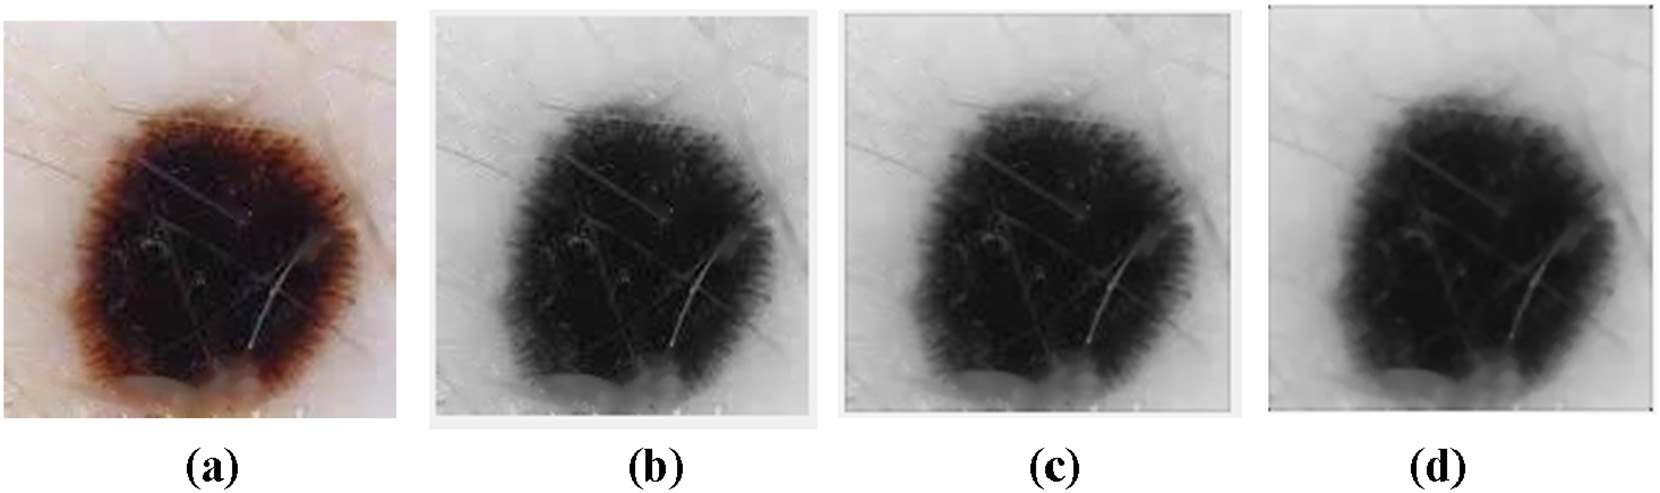
\includegraphics[width=15cm]{./chapter-03-state-of-the-art/preprocessing.png}
\end{center}
\caption{Preprocessing: (a)Dull razor image, (b) Gray scale image, (c) Gaussian filter, (d) Median filter.}
\label{fig:Preprocessing}
\end{figure}




\begin{figure}[htbp]
\begin{center}
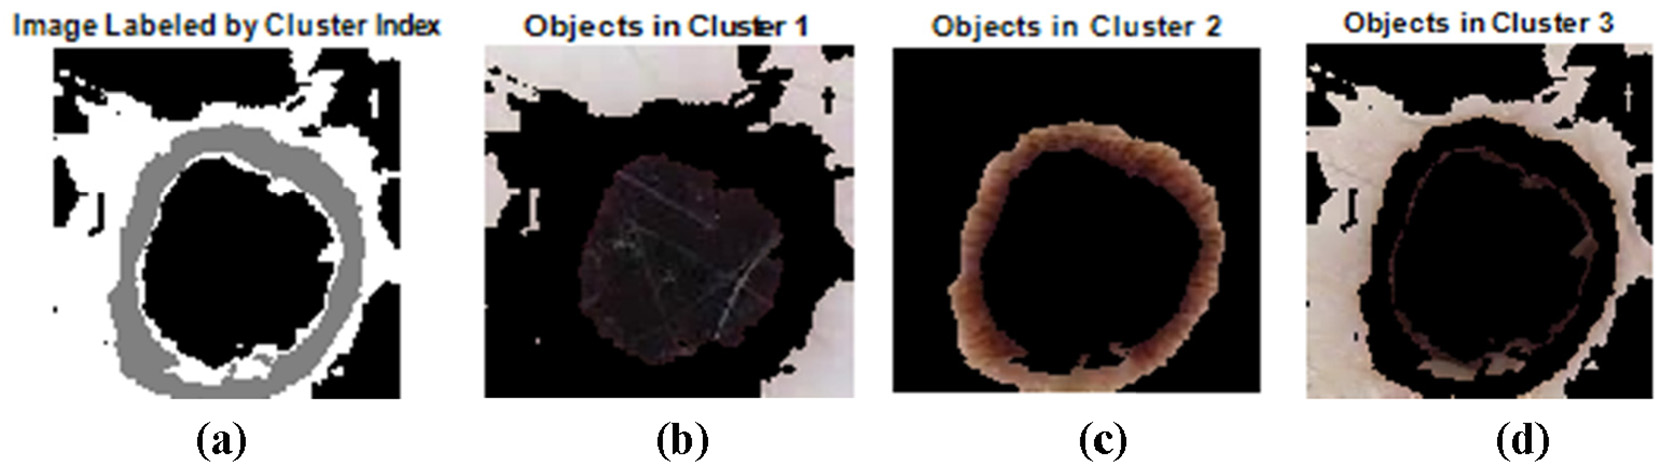
\includegraphics[width=15cm]{./chapter-03-state-of-the-art/segmentation.png}
\end{center}
\caption{Segmentation: (a) Image labelled by cluster index, (b) Objects in cluster 1, (c) Objects in cluster 2, (d) Objects in cluster 3.}
\label{fig:segmentation}
\end{figure}


\begin{figure}[htbp]
\begin{center}
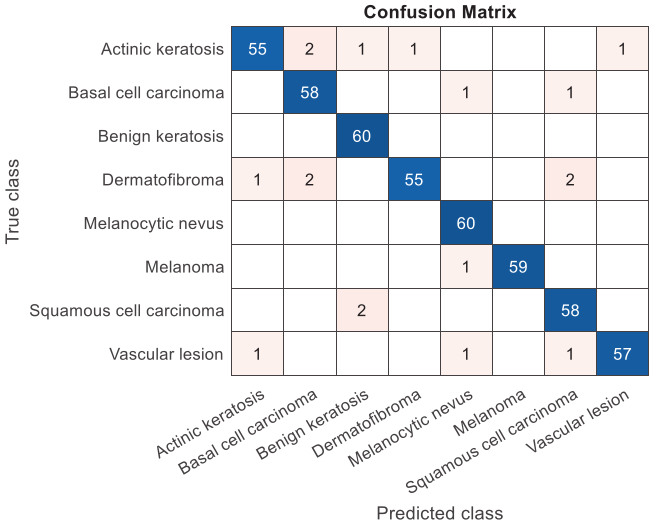
\includegraphics[width=15cm]{./chapter-03-state-of-the-art/confusion-matrix.png}
\end{center}
\caption{Confusion Matrix}
\label{fig:confusion-matrix}
\end{figure}



%=================================================================

\section{Finding reduced Raman spectroscopy fingerprint of skin samples for melanoma diagnosis through machine learning}
    This article ~\cite{Daniella2021} uses a new non invasive approach to classify malignant and benign tumors, and that is by using Raman spectral data instead of images, Raman Spectroscopy is a way to analyse the chemical structure using light and vibrational energy modes of molecules ~\cite{Edinburgh}
\begin{description}
\item[data and method] \hfill \\
    
    \textbf{dataset: }
    for the dataset they brought 33 benign and 51 malignant smaples and cut them into regular cuts of $2mm^3$, a layser was used to excite the samples to collect the Raman signals using special tools after this they aquired 436 Raman spectra. and they focused on the biological fingerprint spectral region from 800 to 1800 $cm^-1$

    \textbf{Fluorescence background data pre-process: }
    Fluorescence is a radiation that is emitted by molecules after interacting with electromagnetic radiation and this could overshdow and disturb the study of Raman spectra, to deal with this noise they used a low frequency laser to lower the probability of fluorescence emissions and by this they could jump the preprocessing step.
\item[feature extraction]
    they divided the obtained spectrums into subsequences (local spectrums) and extracted some statistical measures from it such as arithmetic mean, standard deviation, derivative ...etc

\item[results and discussion]
    these statistical features were then given to a machine learning classification algorithm, a complex dicision tree impimented using lightGBM (open source software), other algorithms were also used such as K-nearest neighbors and XGBOOST (Extreme Gradient Boosting an open source software) but the best performance was obtained using lightGBM.
    further research led them to only use the derivative as a feature and a spectral region from 896 to 1039 $cm^-1$ because these two were proved the most discriminative information between malignant and benign tumors and by this they obtained a high performant model ($AUC \geq 0.97$) shown in figure \ref{fig:roc}
\end{description}

\begin{figure}[htbp]
\begin{center}
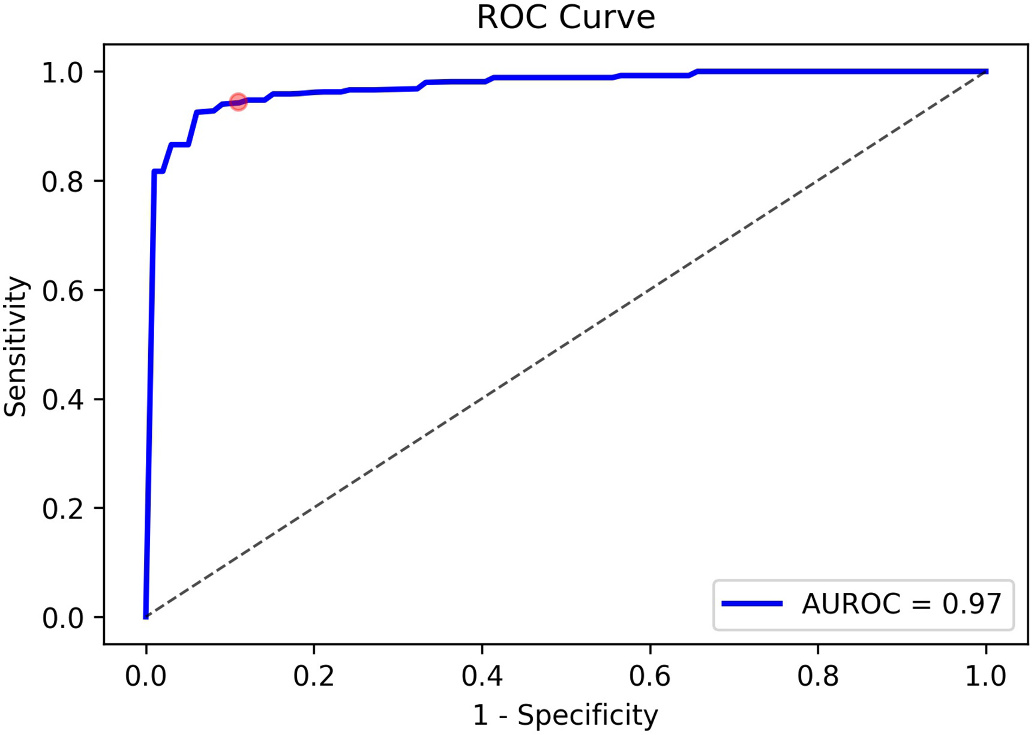
\includegraphics[width=10cm]{./chapter-03-state-of-the-art/ROC.png}
\end{center}
\caption{ROC}
\label{fig:roc}
\end{figure}

% \begin{figure}[htbp]
% \begin{center}
% 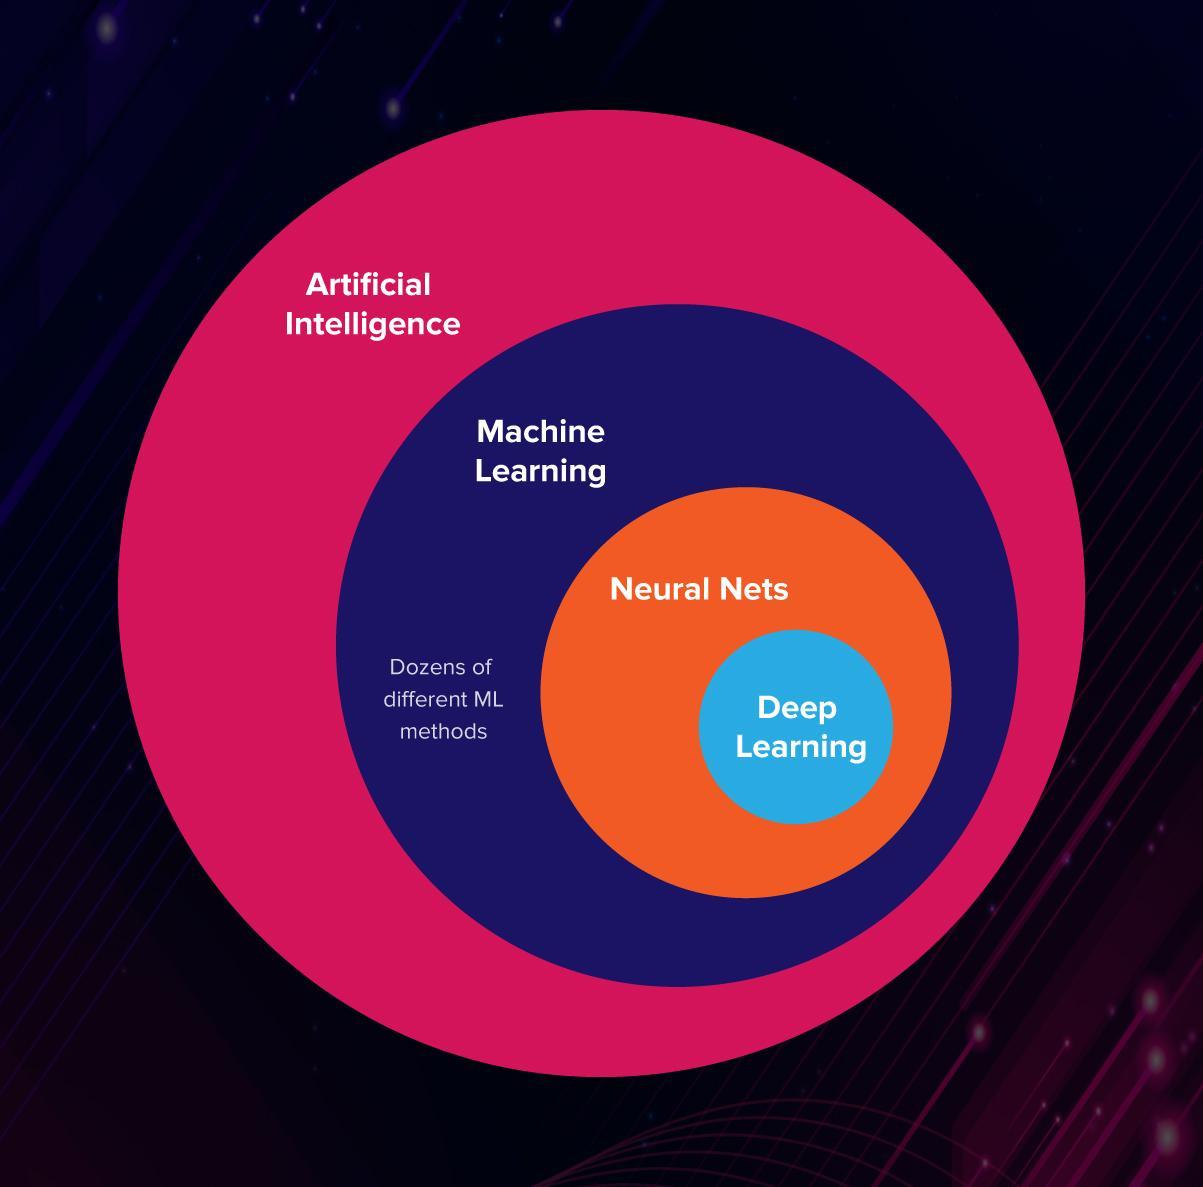
\includegraphics[width=2cm]{./chapter-03-state-of-the-art/versus.jpg}
% \end{center}
% \caption{}
% \label{fig:}
% \end{figure}
